\section{Multi-Layer Perceptron Classifier}\label{sec:MLP}
	    \pagestyle{mario}
	    \sectionauthor{M. Gini \& T. M. Hayden} %\printinunitsof{cm}\prntlen{\linewidth} this shows linewidth in cm

This section presents the multi-layer perceptron (MLP) classifier designed to classify the CIFAR-10 dataset. It is organized as follows: Section \ref{subsec:setup} introduces the software setup used to implement the MLP classifier. Section \ref{subsec:preProp} discusses the data preprocessing and augmentation. Section \ref{subsec:netStruct} analyzes the effect of different network structures on performance. Section \ref{subsec:optNet} analyzes the effect of different hyperparameters.

\subsection{Software Setup}\label{subsec:setup}

MATLAB's Neural Networks toolbox is employed to implement the MLP classifier. The toolbox provides convenient algorithms and applications to design the MLP. A network training function with a convenient graphical user interface (GUI) to observe the progress is included as well. Figure \ref{fig:NNtool} shows the GUI.

Since this is a classification problem, parts of the network structure are given. The output of the MLP should be a prediction of to which class the input belongs to. This is accomplished with the help of the softmax function, also called normalized exponential function. Equation \ref{eq:softmax} shows the formula of such a function. A softmax layer is then used as the last layer. It gets a $K$-dimensional input vector $\boldsymbol{z}$ of arbitrary real values and "squashes" it into a $K$-dimensional output vector $\sigma(\boldsymbol{z})$ of real values in the range $[0,1]$. In our case, $K=10$ and the output values represent the probabilities that the input belongs to the respective class. The class with the highest probability then constitutes the predicition of the MLP.

Every ANN will have at the very least one input layer and one output layer. The size of the input layer simply depends on the size of the input data vector. In the case of CIFAR-10 the input size is $1*3072$, the number of pixels per image.

In addition to the input layer, each network will also have an output layer. The size of the output layer is also defined by the format of the data. In the the case of CIFAR-10, the output layer is a softmax layer with 10 nodes corresponding to each class label.

\begin{equation}\label{eq:softmax}
\sigma(\boldsymbol{z})_j = \frac{e^{z_j}}{\sum_{k=1}^{K}e^{z_k}}\quad \textrm{for}\quad j = 1,...~K.
\end{equation}

\begin{figure}[h!]
  	\centering
  	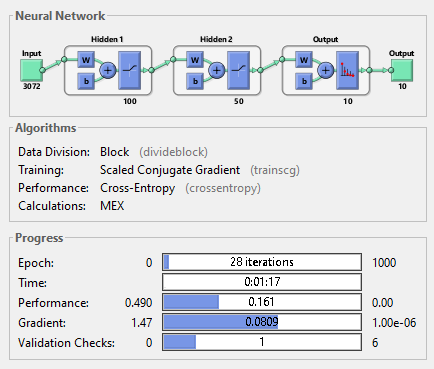
\includegraphics{images/NNtool}
  	\caption{Screenshot of MATLAB's nntraintool.}
  	\label{fig:NNtool}
\end{figure}

The other hidden layers consist of standard MLP. The input to the MLP are the pixel values of the image. Preprocessing and augmentation as described in the next section is also done before the pixel values are fed into the network.

MATLAB offers lots of adjustable settings for the MLP. Unless mentioned otherwise, the following settings are employed as default settings:

\begin{itemize}
	\item Training function: 'trainscg' which is the scaled conjugate gradient method.

	\item Loss function: 'crossentropy' which penalizes

	\item Activation function: 'tansig' which is the hyperbolic tangent sigmoid activation function

	\item The training batch size is set to 20000 images. This constitutes a compromise between a good performance and a reasonable training time.

	\item As a default network structure, two hidden layers are employed with 100 and 50 neurons.

	\item Dataset structure: 80\% are used for the training and 20\% are used for validation. For the testing, the dedicated testing batch provided in the dataset is utilized.

	\item Weight initialization: The weights of the neurons are randmoly initialized. Since this leads to slightly different performances for each run, for the performance analysis each configuration is run five times and then the test accuracy is averaged.
\end{itemize}

\FloatBarrier
\subsection{Data Preprocessing and Augmentation}\label{subsec:preProp}

Data preprocessing and augmentation take place before the data is fed into the network. In the preprocessing step, the data is normalized and centered around the mean. In the augmentation step, the amount of data is augmented through operations like image flipping.

\subsubsection{Data Preprocessing}\label{subsub:dataPreProp}

  	Each image of the dataset is represented by a 32*32*3 array, which results in 1024 pixel values per color channel. To be processed by the MLP, it is transformed into a 1*3072 array. The pixel values are integers in the range [0,255]. For normalization, the data is divided by 255 to lie within the range [0,1]. Accordingly, the datatype changes from the integer type to double. In a second step, the mean per pixel over the whole training set is subtracted. This centers the data per channel.

  	Data preprocessing also includes the division of the complete dataset into appropriate training, validation and test data batches. There are 50000 images available for training. With the default splitting into training and validation dataset (80\% for training and 20\% for validation), Figure \ref{fig:dataPreprocessing} shows the effect of increasing the training batch size as well as employing data preprocessing.

  	\begin{figure}[h!]
  		\centering
   		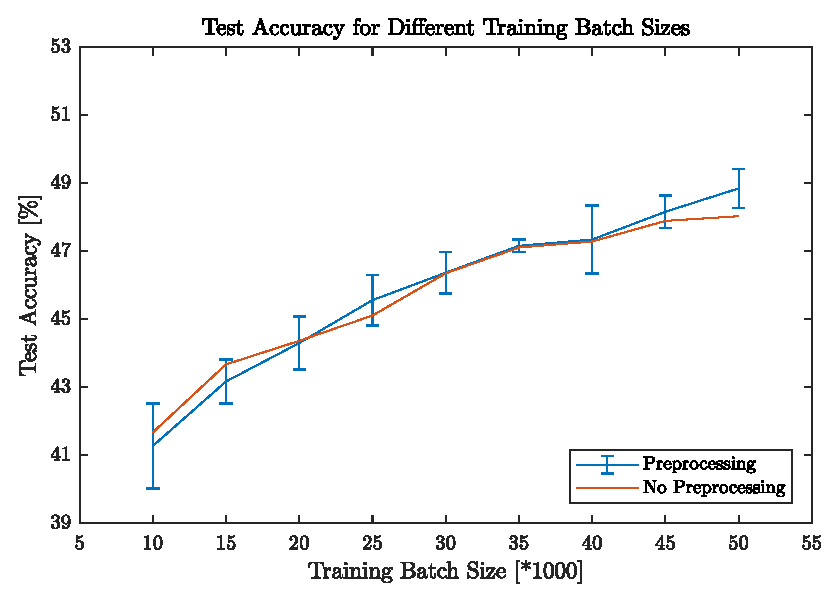
\includegraphics{images/dataPreprocessing}
   		\caption{Comparison of network performance with and without data preprocessing. The errorbars represent one standard deviation.}
   		\label{fig:dataPreprocessing}
   	\end{figure}

   	As intuitively expected, the test accuracy increases for an increasing training batch size. However, the data preprocessing does not lead to a significant increase of performance. The normalization and mean subtraction do not have a big influence in that specific case since the input values already lie in a well defined range and the mean per pixel is also a almost constant value over all pixels. The errorbars show that the different accuracies are most likely due to the random weight initialization.

\FloatBarrier
\subsubsection{Data Augmentation}

Figure \ref{fig:dataPreprocessing} above shows that a larger training batch size leads to an increased performance. A natural approach is therefore to artificially increase the training batch size. Image flipping and image rotation are implemented. Figure \ref{fig:dataAugmentation} illustrates the performance gain from vertical image mirroring. The test accuracy is significantly increased for all training batch sizes by around \SI{3}{\percent}.

   	\begin{figure}[h!]
		\centering
   	  	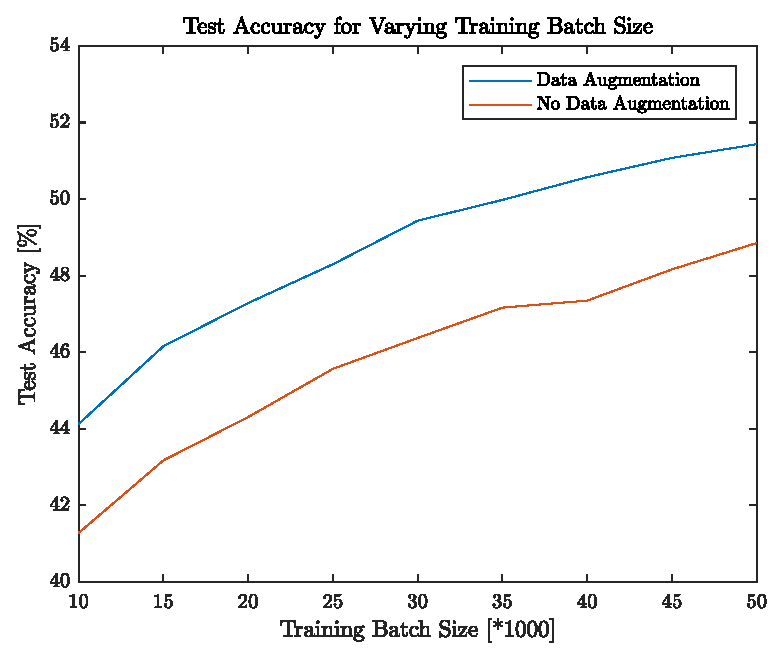
\includegraphics{images/dataAugmentation}
   	  	\caption{Comparison of network performance with and without data augmentation. The errorbars represent one standard deviation.}
   	  	\label{fig:dataAugmentation}
   	\end{figure}

Figure \ref{fig:dataAugDemo} illustrates the data augmentation process on a cat image. The image is mirrored and rotated three times by 90 degrees. This results in a 8-fold increase of the training data size.

   	\begin{figure}[h!]
   		\centering
   		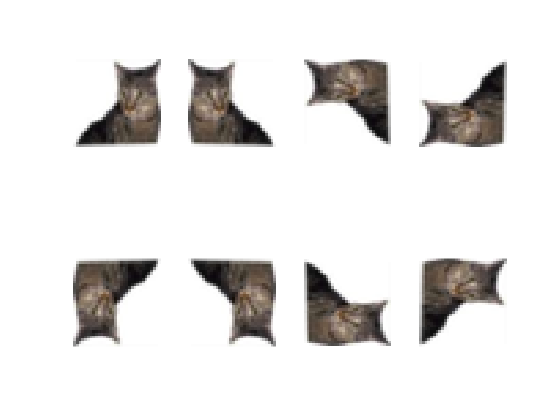
\includegraphics{images/DataAugDemo.png}
   		\caption{Illustration of the data augmentation process on a cat image.}
   		\label{fig:dataAugDemo}
   	\end{figure}


\FloatBarrier

\subsection{Optimization of Network Structure}\label{subsec:netStruct}

Choosing the correct architecture of a neural network remains an area of study which is still not fully understood\cite{andersen1999cross}. For a given problem, there is a variety of valid MLP architectures. Approaches to choose an architecture are mostly based on heuristics and therefore not foolproof\cite{andersen1999cross}.

\subsubsection{Number of Hidden Layers}

In general, a MLP can have an arbitrarily large number of hidden layers. However, MLP architectures with a large number of hidden layers are not common. Additionally, adding more layers increases the chance that the classifier finds a local minimum\cite{de1993backpropagation}. Figure \ref{fig:layers} shows the effect of varying the number of hidden layers of the default MLP classifier. Note that the test accuracy remains almost constant for more than two hidden layers.

\begin{figure}[h!]
    \centering
    \includegraphics{images/numberlayers}
    \caption{Effect of varying the number of hidden layers of the default MLP classifier. The errorbars represent one standard deviation of the averaging process.}
    \label{fig:layers}
 \end{figure}

\subsubsection{Number of neurons per layer in the MLP}

Choosing the optimum number of neurons per layer is a challenging task when designing any MLP architecture. Even in modern archetectures, the number of neurons is generally first estimated using empirical rules and then optimised for the particular dataset\cite{lawrence1998size}. This is especially the case when using noisy datasets such as CIFAR-10.

Figure \ref{fig:surfaceLayers} shows the result of varying the number of neurons per layer on a MLP with two hidden layers. The results show that the number of neurons in the first layer have very little effect on the test accuracy. In addition the results also show that increasing the number of neurons beyond around 70 had very little to no effect. Increasing the number of neurons also increased the time to train. The of neurons in the second layer also had a much stronger impact on the time taken to train than the number of neurons in the first layer.

	\begin{figure}[h!]
   		 \centering
   		 \includegraphics{images/surfacelayers}
   		 \caption{Hello Boy2}
   		 \label{fig:surfaceLayers}
    \end{figure}

\FloatBarrier

\subsection{Optimization of Network Hyperparameters}\label{subsec:optNet}

Hyperparameter selection for ANN such as MLP has become an active field of research with various algorithms being used to estimate optimal parameters\cite{bergstra2011algorithms}. However, since these algorithms rely on performing many trials and updating the parameters accordingly, they proved unsuitable for our purposes due limited computational resources. Instead, a few parameter are varied while using the default MLP structure. Optimal parameters are then estimated from these trends.
%\subsubsection{Learning Rate}
%
%Choosing the learning rate for a MLP classifier can be a challenging process. There is no approach that will work optimally for every dataset. A learning rate that is too high can overshoot the solution and become unstable. However low learning rates can become stuck in local minima or take a long time to train. A good solution is to pick a high learning rate that can pass over local minima and  to gradually decrease the learning rate so that the classifier does not become unstable. This will result in a classifier which initially follows general trends and 'explores' a large portion of the parameter space. Later on the smaller learning rate will allow for the model to be fine tuned into a particular solution.
%
%The effects of changing the learning rate in our model can be seen in Figure \ref{fig:learningRate}. The figure shows that increased learning rates, in general, had a positive effect on model accuracy.
%
%\begin{figure}[h!]
%    \centering
%    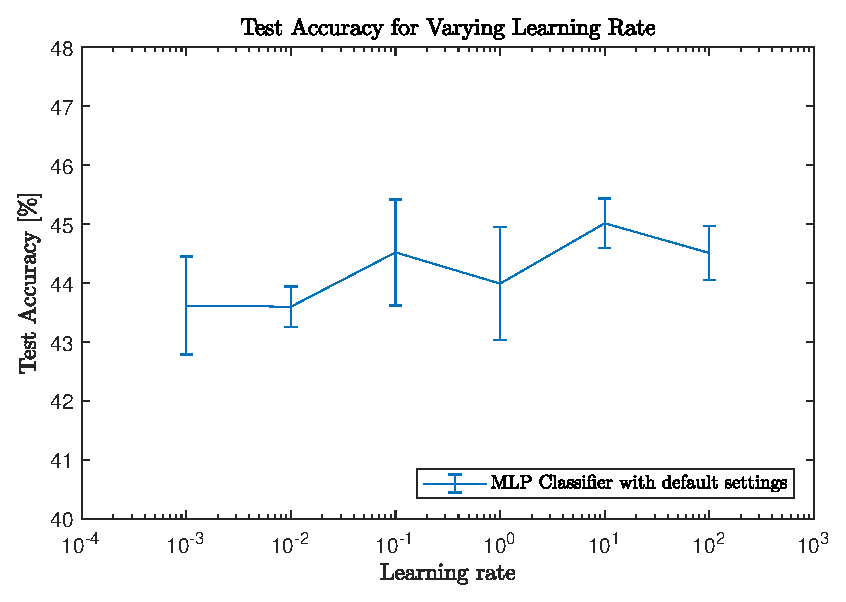
\includegraphics{images/learningRate.eps}
%    \caption{Comparison of the test accuracy of the default MLP using different learning rates.}
%    \label{fig:learningRate}
% \end{figure}
%\FloatBarrier

 \subsubsection{Performance Function}

 The performance function is used to measure the error that a specific input produces in the network. The error expression is then used in the training algorithm which usually is a variation of the backpropagation method\cite{hecht1988theory}. MATLAB offers the following different performance functions:

 \begin{itemize}
 	\item SAE, the sum absolute error function
 	\item SSE, the sum squared error function
 	\item MAE, the mean absolute error function
 	\item MSE, the mean squared error function
 	\item Crossentropy error function
 \end{itemize}

 As Figure \ref{fig:performFct} shows, three performance functions result in a similar performance: MSE, SSE and Crossentropy. SAE and MAE result in a slightly lower performance. An explanation might be that these two functions take the absolute error instead of the squared error. Using the squared error leads to a stronger penalization of larger errors. The best performance is achieved using the crossentropy performance function. This performance function heavily penalizes large errors with very little penalty for small errors. It is also recommended by MATLAB for classification tasks.

 \begin{figure}[h!]
 	\centering
 	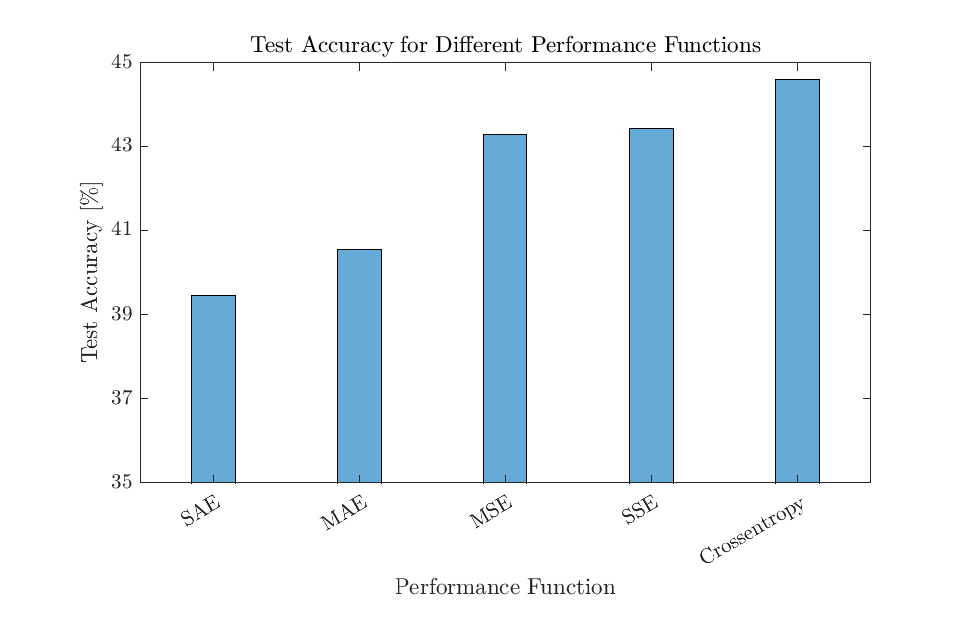
\includegraphics{images/performFct}
 	\caption{Comparison of the test accuracy of the default MLP using different performance functions.}
 	\label{fig:performFct}
 \end{figure}

 \subsubsection{Activation Function}

 The activation function controls the firing of a single neuron. After multiplying the input with the weight and bias vector, the result is fed into the activation function. The output of the activation function constitutes the output of the neuron. Again, MATLAB offers a variety of different activation functions. For the sake of completeness, all activation functions are tested with the default MLP. The result is displayed in Figure \ref{fig:activationFct}.

 \begin{figure}[h!]
 	\centering
 	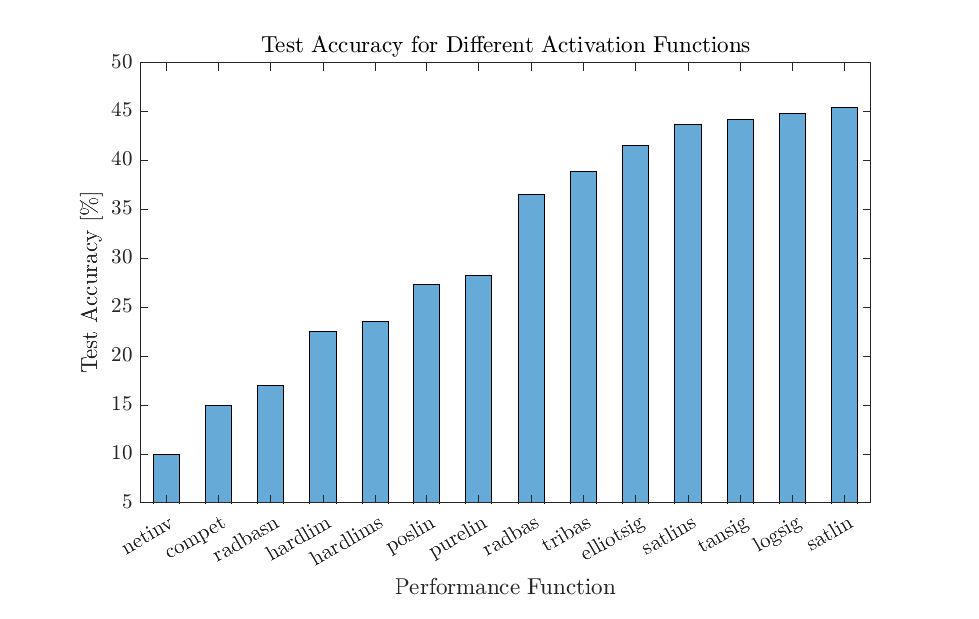
\includegraphics{images/activationFct}
 	\caption{Comparison of the test accuracy of the default MLP using different activation functions.}
 	\label{fig:activationFct}
 \end{figure}

 It can be seen that several activation functions are not suited for a MLP classification problem, e.g the 'netinv' and 'compnet' type. Furthermore, there is a class of activation functions which are very similar and all perform well on that specific problem. Specifically, sigmoid shaped activation functions seem to be the appropriate choice for our problem setting. 'tansig' and 'logsig' are quite similar and 'satlin' and 'satlins' can be viewed as linear approximations of those nonlinear activation functions. It is interesting to note that using the 'satlin' type results in the best performance.

\subsubsection{Training Function}

 The training function is the algorithm that dictates the training process of the network. Once again, MATLAB offers a wide selection of training algorithms. Most are variations of the backpropagation algorithm. Figure \ref{fig:trainingFct} shows the results of using various training algorithms on the default MLP structure.

 \begin{figure}[h!]
 	\centering
 	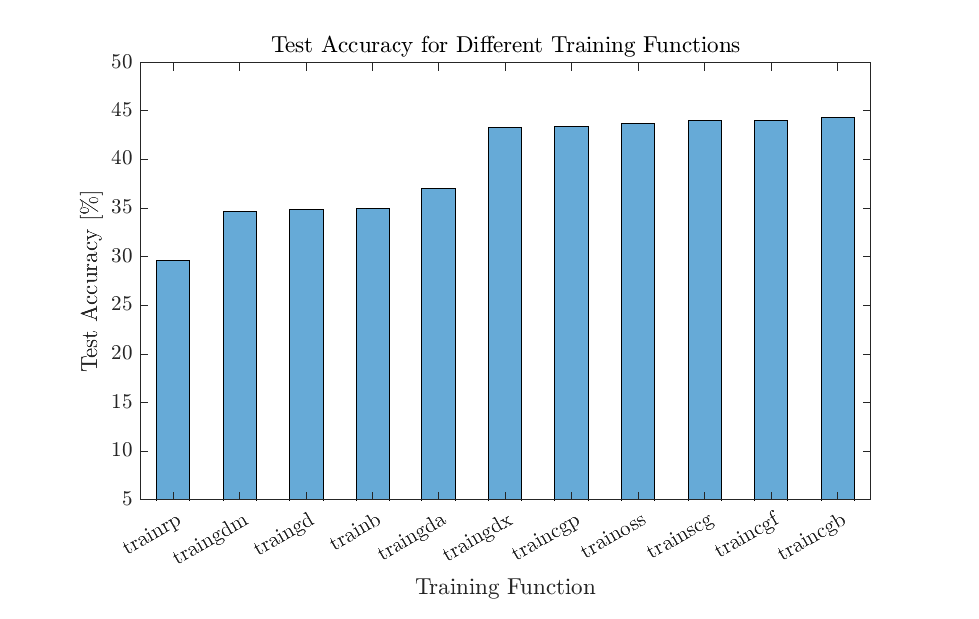
\includegraphics{images/trainingFct}
 	\caption{Comparison of the test accuracy of the default MLP using different training functions.}
 	\label{fig:trainingFct}
 \end{figure}

 All variations of the conjugate gradient backpropagation algorithm\cite{moller1993scaled} achieve good performance. It is interesting that the performance is superior compared to variations of simple gradient backpropagation. 'traindx' which uses momentum is the only gradient backpropagation variation which achieves similar performance than conjugate gradient backpropagation.

 An advantage of conjugate gradient backpropagation algorithms is that they do not require a learning rate parameter. Since our investigations show that they are superior over other backpropagation methods, no further analysis on finding optimal learning rates is conducted.

\subsection{Optimized Classifier}

\begin{figure}[h!]
   \centering
   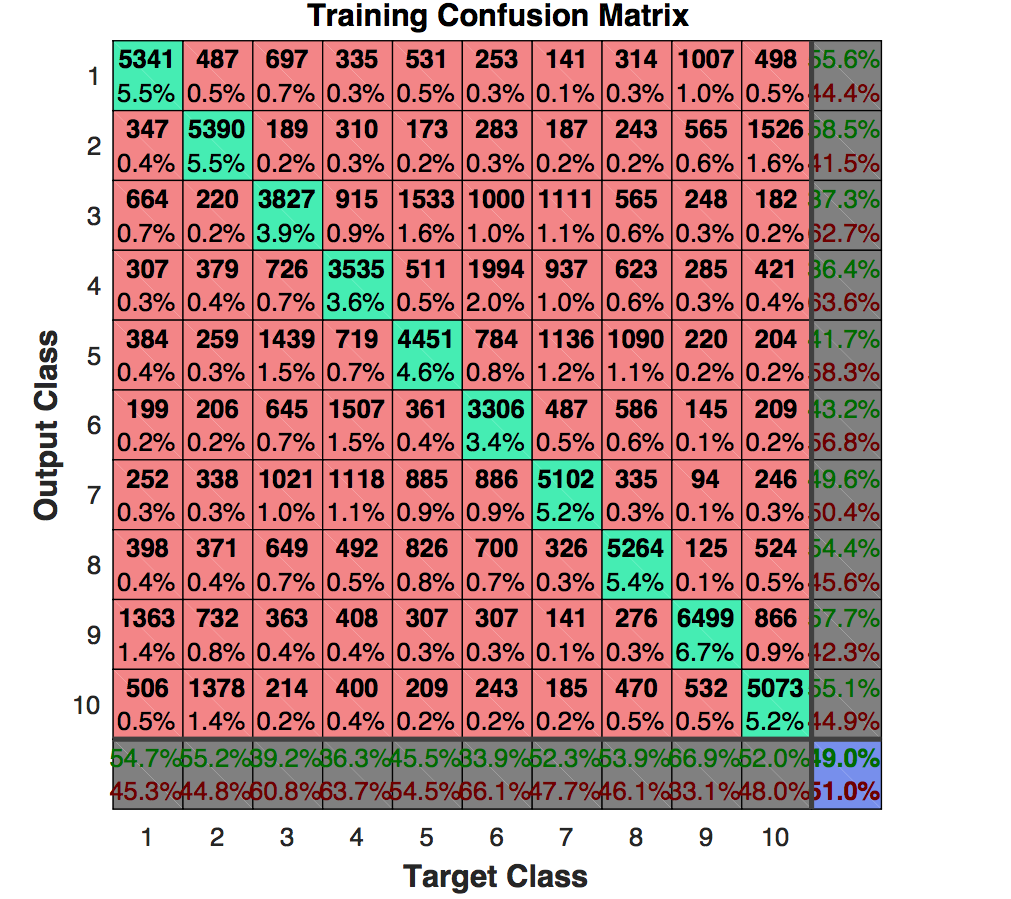
\includegraphics[width=\textwidth]{images/Confusion_Matrix}
   \caption{Confusion Matrix for the final MLP classifier }
   \label{fig:Conf_Matrix}
\end{figure}
